\documentclass[a4paper, oneside]{report}
\usepackage[T1]{fontenc}
\usepackage[utf8]{inputenc}
\usepackage[italian]{babel}
\usepackage{graphicx}
\usepackage{amsmath}
\usepackage{mathtools}
\usepackage{hyperref}
\usepackage{subfigure}
\usepackage{multirow}
\usepackage{listings}
\usepackage{color} %red, green, blue, yellow, cyan, magenta, black, white
\definecolor{mygreen}{RGB}{28,172,0} % color values Red, Green, Blue
\definecolor{mylilas}{RGB}{170,55,241}
\usepackage{caption}
\usepackage{tabularx}
\usepackage{changepage}

\begin{document}

\lstset{language=bash,%
    %basicstyle=\color{red},
    breaklines=true,%
    keywordstyle=\color{black},%
    morekeywords=[2]{1}, keywordstyle=[2]{\color{black}},
    identifierstyle=\color{black},%
    stringstyle=\color{black},
    commentstyle=\color{black},%
    showstringspaces=false,%without this there will be a symbol in the places where there is a space
    numbers=left,%
    numberstyle={\tiny \color{black}},% size of the numbers
    numbersep=9pt, % this defines how far the numbers are from the text
    emph=[1]{sudo, add, wget, systemctl, start, status, apt, key, get,]},emphstyle=[1]\color{black}, %some words to emphasise
    %emph=[2]{word1,word2}, emphstyle=[2]{style},    
}

%%%%%%%%%%%%%%%%%%%%%%%%%%%%%%%%%%%%%%%%%%%%%%%%%%%%%%%%%%%
% copertina

% vspace serve ad aggiungere extra spazio verticale
% em sta ad indicare la grandezza della lettera M maiuscola

% Large indica una dimensione del font di 14.4 pt
% large indica una dimensione del font di 12 pt
% normalsize indica una dimensione del font di 10 pt

% vfill inserisce sufficiente spazio binaco verticalmente per fare in modo che il
% sopra e il sotto del testo siano allieneati col margine superiore e inferiore
\begin{titlepage}
\begin{adjustwidth}{-5em}{}
 \begin{center}
	\vspace{4em}
      {\Large \textsc{Università degli Studi del Sannio}}\\
      \vspace{1em}
      {\Large \textsc{Dipartimento di Ingegneria}}\\
      \vspace{1em}
      {\large \textsc{Corso di Evoluzione e Qualità del Software}}\\
      \vspace{5em}
      {\normalsize \textbf{Analisi dell'Impatto dei Cloni su Technical Debt e Code Smells}\\
      	\vspace{1em}
      	% {\large \textbf{--------------------}}
      }%\\
    \end{center}

\vskip 2.5cm
\begin{center}
	\begin{minipage}[t]{0.5\textwidth}
		\begin{flushleft}
			\large Professoressa:\vspace*{0.2cm} \\
			Aversano Lerina
		\end{flushleft}
	\end{minipage}%
	%
	\begin{minipage}[t]{0.5\textwidth}
		\begin{flushright}
			\large Studenti:\vspace*{0.2cm} \\
			De Luca Lucio 399/168\\
			Grimaldi Gaia 399/162\\
			Laudiero Aurelio 399/167\\
			Tedesco Francesco 399/180\\
		\end{flushright}
	\end{minipage}
\end{center}
\end{adjustwidth}


\vspace*{1.5cm}
\begin{center}
\begin{minipage}[t]{0.5\textwidth}
	{\normalsize Anno Accademico 2018/2019}
\end{minipage}
\end{center}
\end{titlepage}
\date{} 
\thispagestyle{empty}
\tableofcontents
\thispagestyle{empty}
\listoffigures 
\thispagestyle{empty}
\listoftables
\thispagestyle{empty}

\setcounter{page}{0}
\chapter{Obbiettivo}
L'obbiettivo dell'elaborato consiste nell'analizzare i sistemi riportati in \autoref{tabella_sistemi} e di osservare come la presenza di cloni costituisca un peggioramento che impatta sul technical debt e sulla presenza di code smells.
\newcolumntype{C}[1]{>{\centering\arraybackslash}p{#1}}
\begin{table}[h]
\begin{center}
\begin{tabular}{|C{4cm}|C{4cm}|}
\hline
Nome Progetto & Versione\\ \hline
Jabref & 4.3 \\ \cline{2-2}
& 4.2\\ \cline{2-2}
& 4.1\\ \cline{2-2}
& 4.0\\ \hline
DnsJava & 2.1.8 \\ \cline{2-2}
& 2.1.7\\ \cline{2-2}
& 2.1.6\\ \cline{2-2}
& 2.1.5\\ \hline
Fastjson & 1.2.50 \\ \cline{2-2}
& 1.2.40\\ \cline{2-2}
& 1.2.30\\ \cline{2-2}
& 1.2.20\\
\hline
\end{tabular}
\end{center}
\caption{Progetti e relative versioni considerati per l'analisi.}
\label{tabella_sistemi}
\end{table}
\\Verrà effettuato un confronto tra le classi contententi cloni e classi in cui non sono presenti cloni e si confronteranno i risultati ottenuti. Gli strumenti usati a supporto dell'analisi sono i seguenti.
\begin{itemize}
\item Nicad4.
\item SonarCloud.
\item Parser python creati ad hoc.
\end{itemize}
\chapter{Introduzione}
I ricercatori hanno studiato a lungo gli effetti che hanno i cloni sulla gestione, manutenzione ed evoluzione dei sistemi software concludendo che i cloni hanno sia effetti positivi che negativi. Sulla scia di questi studi, in questo elaborato, si andrà ad analizzare l'effetto che hanno i cloni sul technical debt e sull'incremento della presenza dei code smells. Quindi si andranno a confrontare le classi in cui sono presenti i cloni e le classi in cui i cloni sono assenti e si vedrà come varia il technical debt e i code smell. In questo capitolo introduttivo si andrà a dare una breve definizione di cosa sono i cloni, il technical deb e i code smell.
\section{Clone}
Un clone è una sequenza di istruzioni duplicata in più punti di un codice sorgente quindi, questo significa che è stato effettuato un "copia e incolla" del codice in un altro punto della stessa classe oppure in un'altra classe. La presenza di cloni comporta un grave difetto che consiste nel fatto che se viene individuato un bug in un frammento di codice, questo affligge tutti gli altri frammenti di codice duplicati. La risoluzione di questo problema mediante refactoring potrebbe essere problematica a causa della possibilità di introdurre errori. Esistono però diverse motivazioni che spingono gli sviluppatori ad inserire del codice clonato nei sistemi software, in particolare:
\begin{enumerate}
\item	strategia di sviluppo;
\item	benefici di manutenzione;
\item	superare i limiti linguistici sottostanti;
\end{enumerate}
D'altra parte, però, i cloni del codice possono avere gravi conseguenze sulla qualità, la riusabilità e la manutenibilità di un sistema software. In particolare, si ha:
\begin{enumerate}
\item	aumento della probabilità di propagazione dei bug;
\item	aumento della probabilità di introdurre un nuovo bug;
\item	aumento della probabilità di cattiva progettazione;
\item	aumento della difficoltà nel miglioramento/modifica del sistema;
\item	aumento dei costi di manutenzione;
\item	aumento dei requisiti di risorse.
\end{enumerate}
Si hanno quattro tipologie di cloni suddivise in due aree:
\begin{enumerate}
\item Classificazione basata sulla somiglianza testuale:
\begin{itemize}
\item	Tipo I: frammenti di codice identico tranne che per le variazioni negli spazi bianchi (potrebbero anche essere variazioni nel layout) e nei commenti. Non è possibile usare una tecniche di confronto linea per linea per individuarlo.
\item	Tipo II: frammenti strutturalmente/sintatticamente identici ad eccezione delle variazioni di identificatori, letterali, tipi, layout e commenti. I cloni di questo tipo hanno la stessa struttura sintattica.
\item	Tipo III: frammenti copiati con ulteriori modifiche. Le dichiarazioni possono essere modificate, aggiunte o rimosse in aggiunta alle variazioni di identificatori, letterali, tipi, layout e commenti.
\end{itemize}
\item Classificazione basata sulla somiglianza funzionale: se le funzionalità dei due frammenti di codice sono identiche o simili, cioè hanno condizioni pre e post simili, si parla di cloni semantici e questi vengono identificati come cloni di tipo IV.
\begin{itemize}
\item	Tipo IV: due o più frammenti di codice che eseguono lo stesso calcolo ma implementati attraverso diverse varianti sintattiche. 
\end{itemize}
\end{enumerate}
La complessità analitica e la sofisticazione nel rilevare i cloni aumenta dal Tipo I al Tipo IV. Il rilevamento dei cloni di tipo IV è quindi il più difficile.\\
Sebbene in generale ci siano solo quattro tipi di cloni, vengono usati termini diversi quando ci si riferisce ai cloni stessi:
\begin{itemize}
\item	exact clones: per fare riferimento ai frammenti di codice identici. Tipicamente clone di tipo I;
\item	near-Miss Clones: per fare riferimento a frammenti di codice identici con dichiarazioni aggiunte, cancellate e/o modificate. Fondamentalmente, tutti i cloni di Tipo II sono cloni near-miss;
\item	renamed clones: quando nomi di identificatori, valori letterali, commenti o spazi bianchi modifiche nei frammenti copiati. Essenzialmente un clone di tipo II;
\item	parametrized clone (o p-match): è un clone rinominato con sistematica ridenominazione. Un sottoinsieme di cloni di tipo II.
\end{itemize}
L'analisi dei cloni è stata effettuata mediante l'uso del software Nicad che consente l'estrazione dei cloni di tipo I, II e III. L'output ottenuto da Nicad è stato manipolato attraverso un parser scritto in python per estrapolare solo le informazioni d'interesse.



\section{Technical Debt}
Il technical debt, conosciuto anche come code debt, è la spesa totale che un'organizzazione paga a causa di un'architettura inadeguata o di processi di sviluppo del software inefficienti. Se il debito non viene risolto continua ad accumulare interesse rendendo così più problematico implementare i cambiamenti futuri. Diversi fattori rendono sempre più difficile la gestione o l'aggiornamento del codice sorgente, inclusa la complessità dell'architettura e le pratiche di sviluppo. I fattori che contribuiscono all'incremento del technical debt sono:
\begin{itemize}
\item pressioni aziendali;
\item processi insufficienti;
\item funzioni hard-coded;
\item insiemi di test scadenti;
\item documentazione di codice scadente;
\item mancanza di collaborazione;
\item refactoring differito.
\end{itemize}
Le date di rilascio aggressive fanno sì che le modifiche vengano ignorate o messe in attesa ed inoltre, le funzioni hard-coded creano applicazioni non flessibili che è impossibile aggiornare nei tempi previsti. Codice scarsamente documentato, test insufficienti e comunicazione minima aumentano il technical debt in quanto il team deve dedicare più tempo per trovare o per risolvere problemi dopo il rilascio.\\ 
Lo strumento utilizzato per analizzare il technical debt è SonarCloud cioè la versione online di SonarQube. SonarQube, e di conseguenza SonarCloud, utilizza il metodo SQALE per calcolare il technical debt. Tale metodo è basato esclusivamente su regole e questo significa che se si vuole gestire tutto il technical debt con SQALE, bisogna prima abilitare le regole nel repository Common SonarQube che contrassegna:
\begin{itemize}
\item blocchi duplicati;
\item casi di test falliti;
\item numero di casi di test insufficiente a coprire i branch;
\item densità di commenti insufficiente;
\item numero di test insufficiente a coprire le linee di codice;
\item casi di test saltati.
\end{itemize}
Tali regole si trovano nel repository Common SonarQube perché sono comuni a tutte i linguaggi di programmazione. Una volta abilitate è possibile tenere traccia di tutti i difetti di qualità e monitorare il debito tecnico, che il metodo SQALE misura in giorni.
\subsection{Il metodo Sqale}
Il metodo SQALE è stato sviluppato per rispondere a un'esigenza generica e permanente di valutazione della qualità del codice sorgente visto che standard come ISO 9126 e ISO / IEC 15939 non forniscono un supporto efficace. Si tratta di un metodo generico ed indipendente da linguaggio e strumenti. Esso permette di:
\begin{itemize}
\item definire chiaramente cosa crea il debito tecnico;
\item stimare correttamente il debito;
\item analizzare tale debito dal punto di vista tecnico e di business;
\item offrire strategie di prioritizzazione diverse che consentono di stabilire un piano di ammortamento ottimale. 
\end{itemize}
Il modello di qualità SQALE viene utilizzato per formulare e organizzare i requisiti non funzionali relativi alla qualità del codice. È organizzato in tre livelli gerarchici:
\begin{enumerate}
\item il primo livello è composto da caratteristiche;
\item il secondo di sotto-caratteristiche;
\item il terzo livello è composto da requisiti relativi agli attributi interni del codice sorgente.
\end{enumerate}
Tali requisiti di solito dipendono dal contesto e dalla lingua del software. Qualsiasi violazione di questi requisiti induce il debito tecnico.
\section{Code Smell}
Il termine Code Smell è stato coniato per la prima volta da Kent Beck e nell’Ingegneria del Software indica codice sorgente che, nonostante sia funzionante, presenta delle imperfezioni logiche che ne riducono la qualità. Non si tratta di veri e propri errori ma la loro presenza può rallentare la manutenzione del software e rendere difficile la  scoperta di bug. \\
Quando ci si accinge a progettare un nuovo software è conveniente definirne una struttura facilmente comprensibile, in maniera tale da garantire flessibilità in caso di aggiunte al codice da effettuare in un secondo momento. I Code Smells incrementano il Software decay, cioè il decadimento del Software a causa della poca manutenzione effettuabile su di esso. La metodologia che permette la correzione di questi prende il nome di Refactoring. 
%I code smell sono parti di codice sorgente caratterizzate da difetti di programmazione; non sono definibili come veri e propri errori. La loro presenza non causa problemi direttamente al funzionamento del software, però possono rallentare la manutenzione del software e rendere difficile la  scoperta di bug. 
SonarCloud consente, in base alle regole settate nel quality profile, di individuare diverse tipologie di smells come ad esempio:
\begin{itemize}
\item "==" and "!=" should not be used when "equals" is overridden
\item "@CheckForNull" or "@Nullable" should not be used on primitive types
\item "@Deprecated" code should not be used
\item "@EnableAutoConfiguration" should be fine-tuned
\item "@Import"s should be preferred to "@ComponentScan"s
\item "@Override" should be used on overriding and implementing methods
\end{itemize}
Ad ognuno viene associato un diverso tipo di severità, in particolare si ha:
\begin{enumerate}
\item blocker;
\item major;
\item info;
\item critical;
\item minor.
\end{enumerate}
In base alla severità viene associato un certo Technical Debt.
\chapter{Tools}\label{cap3}
Al fine di analizzare l'impatto dei cloni sul \textbf{technical debt} e sui \textbf{code smells} sono stati utilizzati i seguenti tools:
\begin{itemize}
\item Nicad Clone Detector, illustrato nella sezione \ref{nicad}
\item SonarCloud, illustrato nella sezione \ref{sonar}
\end{itemize}
\section{Nicad}
NiCad Clone Detector è uno strumento scalabile e flessibile per l'individuzione dei cloni basato su Txl e progettato per implementare il NiCad hybrid clone detection method. Quest'ultimo è un metodo ibrido che combina language-sensitive parsing con language-independent similarity analysis per identificare cloni significativi.
Il metodo comprende tre fasi principali: il parsing, la normalizzazione e il confronto.
Nella prima fase le sorgenti di input vengono parsate per poter estrarre tutti i frammenti, come ad esempio funzioni o blocchi, di una data granularità. Ogni frammento estratto è un potenziale clone e su di esso vengono effettuate alcune operazioni: spaziature e interruzioni di linee vengono normalizzati e i commenti vengono rimossi. 
Nella seconda fase, i frammenti estratti vengono normalizzati, filtrati o astratti prima del confronto. Ad esempio, possono essere trasformati rinominandoli o rimuovendo le dichiarazioni.
Nell'ultima fase, i frammenti normalizzati ed estratti sono confrontati a livello lineare usando un algoritmo LCS (Longest Common Subsequence) ottimizzato per rilevare i frammenti simili, ovvero i cloni. Il confronto è parametrizzato utilizzando una soglia di differenza che consente un rilevamento più o meno accurato. Ad esempio, una soglia di differenza 0.0 rileva solo i cloni esatti, 0.1 rileva quelli che possono differire del 10\%, 0.2 fino al 20\% e così via.

E'\ progettato per essere utilizzato via linea di comando Linux, Solaris, Cygwin o MAc OSs definendo la granularità desiderata dell'elaborazione e la directory del sorgente da analizzare, per esempio: 

\begin{center}
\verb|nicad functions java examples/dnsjava-2.1.8|
\end{center}

Nicad supporta due granularità, ossia funzioni (functions) e blocchi (blocks) e cinque linguaggi: C, C\#, Java, Phyton e WSDL.
Di default effettua il confronto senza normalizzare, filtrare o ridenominare trovando semplicemente cloni esatti o near-miss a quattro soglie di differenza: 0.0, 0.1, 0.2, e 0.3 che corrisponde allo 0\%, 10\%, 20\% e 30\% di linee diverse nei frammenti estratti.
L'output è costituito da un file XML ed un file HTML, memorizzati nella stessa cartella in cui è presente il sorgente. 
Per specificare la normalizzazione, il filtraggio e la ridenominazione si aggiunge il nome del file di configurazione a linea di comando:

\begin{center}
\verb|nicad functions java examples/dnsjava-2.1.8 type2|
\end{center}

In questo caso, si utilizza il file di configurazione "type2.cfg".
I file di configurazione consentono all'utente di specificare una gamma di opzioni, come ad esempio la dimensione massima o minima dei cloni, la ridenominazione o le normalizzazioni da eseguire. Ogni opzione specificata in questi file invoca un plugin NiCad che viene eseguito prima del confronto tra i potenziali cloni. I plugin sono implementati in TXL e l'utente può anche aggiungere nuove normalizzazioni programmandole con questo linguaggio.






 \label{nicad}
\section{SonarCloud}\label{sonar}
\textbf{SonarCloud} \footnote{https://sonarcloud.io} è il prodotto leader per la \textbf{Continuous Code Quality} online ed è completamente gratuito per progetti open-source. Supporta tutti i principali linguaggi di programmazione, inclusi Java, C\#, JavaScript, C/C++ e molti altri. \textbf{SonarCloud} offre integrazioni end-to-end per i team che sfruttano le seguenti soluzioni nei loro processi di sviluppo:
\begin{itemize}
	\item GitHub
	\item Bitbucket Cloud
	\item Azure DevOps
\end{itemize}
Consente di effettuare le stesse analisi possibili in SonarQube \footnote{https://www.sonarqube.org/} senza però avere la necessità di installare il servizio in locale.
\subsection{SonarQube runner}
\textbf{SonarCloud} attualmente non triggera l'analisi automaticamente ma è necessario avviarla all'interno di uno script di \textbf{Continuous Integration} utilizzando uno tra i seguenti scanner disponibili:
\begin{itemize}
	\item SonarScanner per Gradle
	\item SonarScanner per MSBuild
	\item SonarScanner per Maven
	\item SonarScanner per Ant
	\item SonarScanner	
\end{itemize}
L'ultimo tra quelli elencati, \textbf{SonarScanner}, può essere utilizzato quando nessuno degli altri risulta appropriato. La scelta è ricaduta su quest'ultimo visto che i progetti analizzati non utilizzano tutti lo stesso \textbf{build automation tool}. 
\subsection{Installazione SonarQube Scanner}
\textbf{SonarQube scanner} è stato utilizzato su una macchina Ubuntu $16.04$ seguendo i passi riportati per l'installazione:
\begin{itemize}
	\item download dal maven repository utilizzando il seguente comando: 
	\begin{verbatim}
		wget 
		http://repo1.maven.org/maven2/org/codehaus/
		sonar/runner/sonar-runner-dist/2.4/sonar-runner-dist-2.4.zip
	\end{verbatim}	
	\item unzip del file utilizzando il comando
	\begin{verbatim}
	unzip sonar-runner-dist-2.4.zip
	\end{verbatim}
	\item è necessario poi rendere eseguibile lo scanner presente nella directory bin utilizzando il comando 
	\begin{verbatim}
			sudo chmod u+x bin/sonar-scanner
	\end{verbatim}
	\item infine si crea un link simbolico in modo tale da poter eseguire lo scanner senza specificare ogni volta il path
	\begin{verbatim}
	 ln -s /opt/sonar-runner/bin/sonar-runner /usr/local/bin/sonar-runner
	\end{verbatim}
\end{itemize}
Risulta poi fondamentale modificare il file di configurazione di \textbf{SonarScanner}, \textit{sonar-scanner.properties}, specificando il seguente campo:
\begin{verbatim}
	sonar.host.url=https://sonarcloud.io
\end{verbatim}
Nel caso di utilizzo di \textbf{SonarQube} in locale, il campo appena specificato dovrà essere modificato nel modo seguente:
\begin{verbatim}
sonar.host.url=http://localhost:9000
\end{verbatim}

\subsection{Configurazione SonarCloud}
Affinché possa essere eseguita l'analisi è necessario configurare \textbf{SonarCloud}. Innanzitutto bisogna effettuare il log-in utilizzando l'account \textbf{gitHub} come mostrato in \autoref{fig:login}. Il secondo passo consiste nel creare un'organizzazione, come mostrato in \autoref{fig:organizzazione}, che sostanzialmente è uno spazio all'interno del quale i membri di un team possono collaborare. Le organizzazioni possono essere create gratuitamente ma i progetti e le analisi risultano pubbliche. \'E possibile anche creare organizzazioni private ma non gratuitamente. Una volta creata un'organizzazione è possibile, come mostrato in \autoref{fig:membri}, aggiungere membri al team specificando l'indirizzo e-mail o il nome utente utilizzato in gitHub dal collaboratore, e creare nuovi progetti. Si mostrano in \autoref{fig:nostraOrg} i membri dell'organizzazione realizzata per il progetto in esame.
\begin{figure}[htbp]
	\centering
	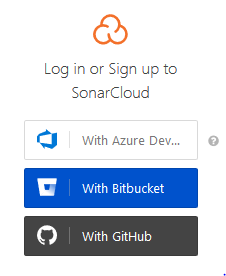
\includegraphics[scale=1, trim = 0cm 0cm 0cm 0cm, clip=true]{figSonarCloud/figLogInSonar.PNG}
	\caption{Schermata Log in SonarCloud}
	\label{fig:login}
\end{figure}

\begin{figure}[htbp]
	\centering
	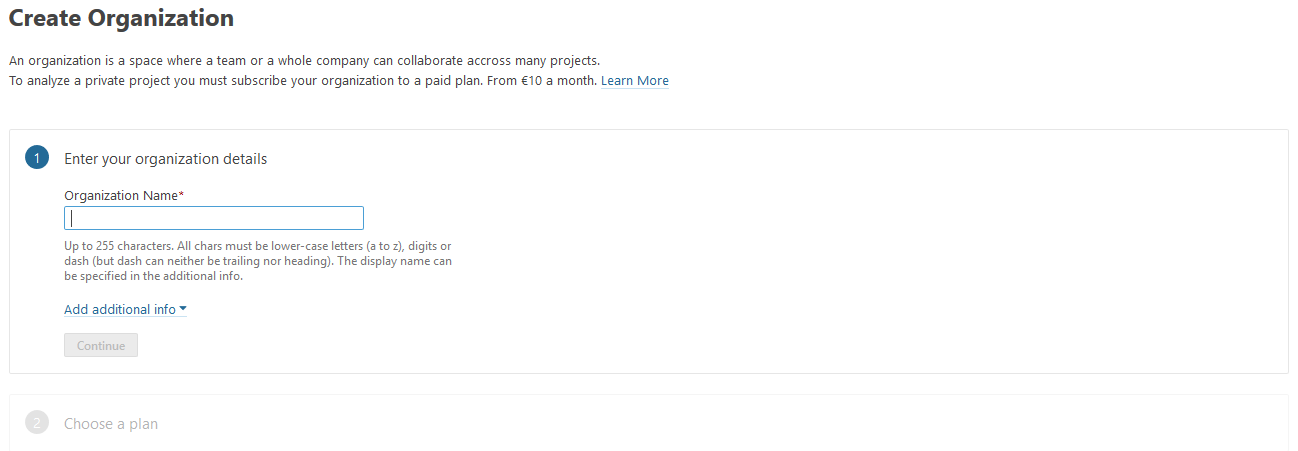
\includegraphics[scale=0.3, trim = 0cm 0cm 0cm 0cm, clip=true]{figSonarCloud/organizzazione.PNG}
	\caption{Creazione di una organizzazione in SonarCloud}
	\label{fig:organizzazione}
\end{figure}

\begin{figure}[htbp]
	\centering
	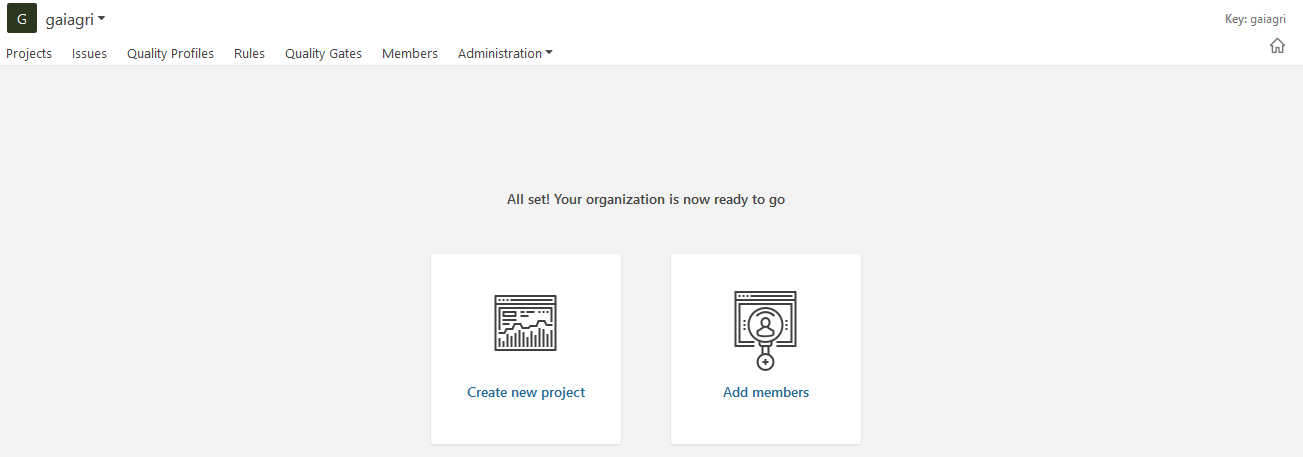
\includegraphics[scale=0.3, trim = 0cm 0cm 0cm 0cm, clip=true]{figSonarCloud/aggiuntaMembri.PNG}
	\caption{Aggiunta membri organizzazione e creazione progetto in SonarCloud}
	\label{fig:membri}
\end{figure}

\begin{figure}[htbp]
	\centering
	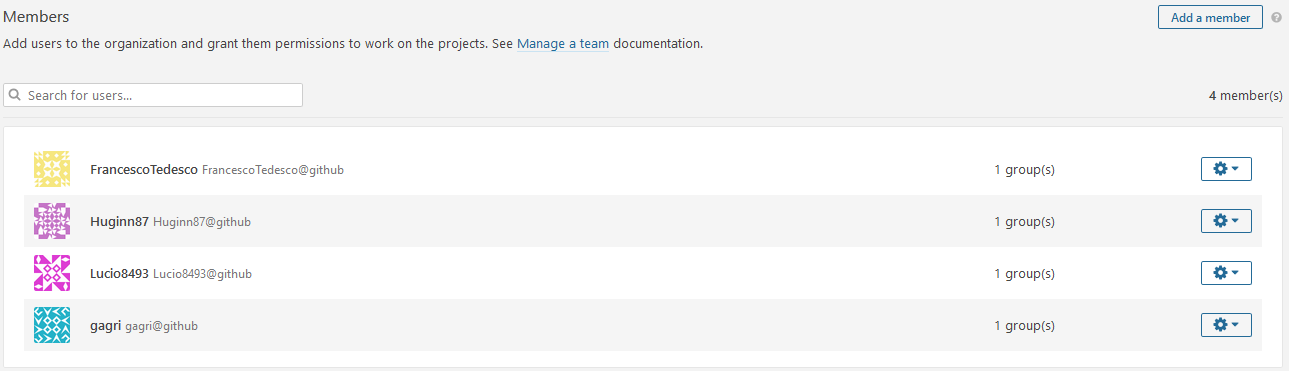
\includegraphics[scale=0.3, trim = 0cm 0cm 0cm 0cm, clip=true]{figSonarCloud/nostraOrganizzazione.PNG}
	\caption{Organizzazione progetto in esame}
	\label{fig:nostraOrg}
\end{figure}
A questo punto è possibile creare un nuovo progetto. E necessario specificare il nome dell'organizzazione, del progetto (che sarà lo stesso utilizzato in gitHub), ed una chiave che sarà univocamente assegnata a quel determinato progetto. Si mostra tale procedura in \autoref{fig:prog}.

\begin{figure}[htbp]
	\centering
	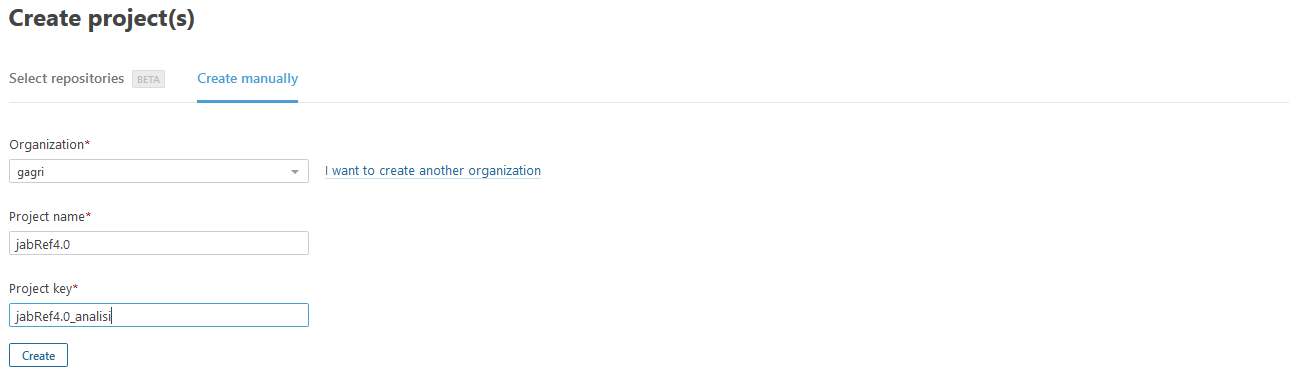
\includegraphics[scale=0.3, trim = 0cm 0cm 0cm 0cm, clip=true]{figSonarCloud/progetto.PNG}
	\caption{Creazione progetto sonarCloud}
	\label{fig:prog}
\end{figure}
Una volta creato il progetto, sarà mostrata una pagina che chiederà se si vuole generare un nuovo token oppure utilizzarne uno esistente. Il token è necessario al file di identificare l'utente che lancia l'analisi. L'associazione tra le informazioni (ossia organizzazione, chiave del progetto e token) e l'utente autorizzato a lanciare l'analisi, viene effettuata attraverso il file \textit{sonar-project.properties} che deve essere presente all'interno del progetto. In particolare, le informazioni contenute sono le seguenti:
\begin{itemize}
	\item 	sonar.projectKey: chiave del progetto
	\item 	sonar.organization: nome dell'organizzazione
	\item 	sonar.host.url: nel caso in cui si utilizza sonarCloud è necessario specificare l'URL di quest'ultimo ossia \url{https://sonarcloud.io}. Nel caso di utilizzo di SonarQube in locale, bisognerebbe specificare \url{http://localhost:9000}
	\item 	sonar.login: token fornito in fase di creazione del progetto
	\item sonar.sources: directory contenete i sorgenti
	\item sonar.java.binaries: directory contenete i binari
	\item sonar.language: linguaggio di programmazione del progetto in analisi
\end{itemize}


A questo punto, basta lanciare il comando 
\begin{verbatim}
sonar-runner
\end{verbatim}
per avviare l'analisi ed una volta che questa è terminata il risultato sarà visualizzabile online come mostrato a titolo esemplificativo in \autoref{fig:analisi}.
	
\begin{figure}[htbp]
	\centering
	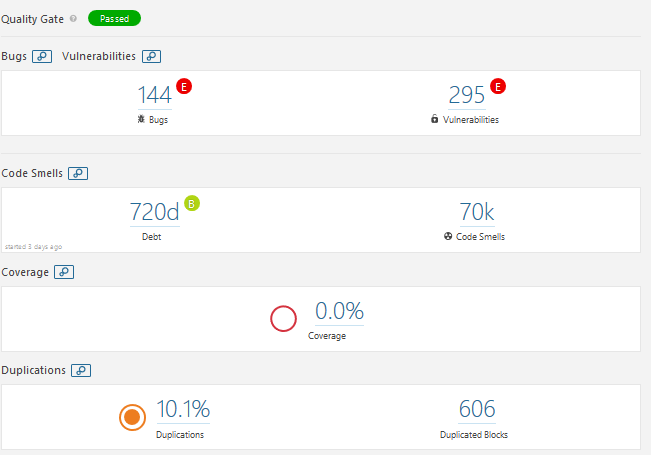
\includegraphics[scale=0.5, trim = 0cm 0cm 0cm 0cm, clip=true]{figSonarCloud/analisi.PNG}
	\caption{Esempio risultato analisi SonarCloud}
	\label{fig:analisi}
\end{figure}

\textbf{SonarCloud}, al pari di \textbf{SonarQube}, consente di configurare i \textbf{Quality Profiles} e i \textbf{Quality Gates}, ossia l' insieme di regole che definiscano il livello di qualità che deve essere rispettato dal progetto in analisi. Nel caso in cui tali regole non siano rispettate, il risultato sarà il fallimento dell'analisi. E'\ possibile utilizzare le regole di default. 

\subsection{SonarCloud Web API}
\textbf{SonarCloud} fornisce una Web API per recuperare le informazioni relative ad un determinato progetto, restituendole in formato JSON. L'API utilizza i classici metodi HTTP come GET , POST e DELETE per identificare il tipo di azione che deve essere realizzata. 

A titolo esemplificativo si mostra una query di richiesta:
\begin{verbatim}
https://sonarcloud.io/api/measures/component_tree?
component=keyJabref4.2&metricKeys=sqale_index&ps=100&p=1
\end{verbatim}

in cui:
\begin{itemize}
	\item \textit{component} rappresenta la chiave del progetto
	\item \textit{metricKeys} indica la metrica che deve essere presa
	\item \textit{ps} indica la page size quindi il numero di elementi. Tale numero può essere cpmpreso tra 0 e 499
	\item \textit{p} indica la pagina. Ad esempio, per progetti di 1500 classi è necessario salvare prima i valori con $p=1$, poi con $p=2$ e poi con $p=3$ ogni volta con $ps=499$.
\end{itemize}

I dati ottenuti sono relativi al Technical Debt. Il parametro specificato è infatti \textit{sqale\_index} che è appunto il metodo utilizzato per misurare il Technical Debt stesso.  

\chapter{Analisi dei Dati}\label{cap4}
\section{Elaborazione Dati Nicad}
Le informazioni relative al codice clonato sono state estratte mediante l'uso di Nicad. Il tool è stato invocato a linea di comando attraverso il comando:
\begin{verbatim}
./nicad functions java directory/Sistema type1
\end{verbatim}
Si nota che:
\begin{itemize}
	\item il primo parametro indica il livello di granularità a cui eseguire l'analisi;
	\item il secondo parametro indica il linguaggio in cui è scritto il sistema sotto analisi;
	\item il terzo parametro specifica il path del progetto
	\item il quarto parametro indica il file di configurazione da utilizzare nell'analisi.
\end{itemize}
Il file di configurazione consente di specificare il tipo di clone da individuare. Facendo variare il file di configurazione è stato possibile ottenere, come output, dei file XML relativi ai diversi tipi di cloni. Nicad ad ogni invocazione produce due file XML:
\begin{itemize}
	\item il primo contiene le coppie di cloni accompagnate da una serie di informazioni tra cui: un ID, la startline, la endline, etc;
	\item il secondo file contiene lo stesso tipo di informazioni, ma riunisce i cloni per classi e non per singole coppie.
\end{itemize}
A partire da questa collezione di file XML si è proceduto a costruire un file CSV che fosse in grado di riassumere tutte le informazioni desiderate. Tale operazione è stata effettuata attraverso un parser\footnote{ParserXML.py} che preleva le informazioni d'interesse, in particolare sono state estratte le seguenti informazioni:
\begin{itemize}
\item l'identificativo della classe
\item l'identificativo del singolo clone
\item il path del file
\item la startline
\item la endline
\item e la similarità
\end{itemize} 
È stata aggiunta anche la versione del sistema analizzato e il tipo di clone. 
È stato creato un ulteriore parser\footnote{ParserCSV.py} che consente di rimuovere gli errori di classificazione commessi da Nicad. Quest'ultimo, infatti, tende a classificare alcuni cloni come afferenti a più tipi. Ad esempio, può classificare un clone di tipo 1 anche come clone di tipo 2 e 3. Il parser identifica i cloni ripetuti e li elimina dal tipo superiore. Ad esempio, se un clone viene identificato come tipo 1 e 2 il parser procede all'eliminazione del clone di tipo 2.
\section{Elaborazione Dati SonarCloud}
La quantita' di informazioni e metriche fornite da SonarCloud risulta enorme rispetto a quelle che possono essere sfruttate al fine dell'analisi d'interesse. Per questo motivo a partire dalle analisi effettuate da SonarCloud si sono prelevate solo le due metriche d'interesse:
\begin{itemize}
	\item \textbf{Il Technical Debt} 
	\item \textbf{I Code Smell}
\end{itemize}
Tali informazioni sono legate al singolo file del sistema, e per questo e' possibile associarle all'analisi fornita da Nicad, nelle quali ad ogni clone e' associato il file su cui si trova. Per ogni sistema d'interesse, si e' proceduto ad analizzare le versioni selezionate in maniera indipendente. Il prelievo effettivo delle informazioni e' avventuo attraverso un semplice copia e incolla su un file di testo. Si e' preferito utilizzare questa procedura per via della semplicita' di informazioni da recuperare, sebbene la WebAPI di SonarCloud consenta il prelievo di informazioni aggregate.
In particolare sono stati creati due file testuali, uno contente la lista del path dei file del sistema e il rispettivo Technical Debt, mentre l'altro associa i Code Smell e i path dei file. Attraverso due parser, ParserDebt.py e ParserSmell.py, e' stato un file CSV che associa ad ogni file, di ogni versione dei sistemi analizzati i corrispettivi Technical Debt e Code Smell.
\section{Analisi dei Dati}
La prima analisi effettuata sui dati ricavati dall'elaborazione dei risultati ottenuti da \textbf{Nicad} e \textbf{SonarQube} ha riguardato il numero di cloni sulle $4$ versioni di ogni progetto. I risultati hanno evidenziato che al crescere della versione la presenza di cloni aumenta, in particolare:
\begin{itemize}
	\item in \textbf{DnsJava}, come mostrato in \autoref{fig:nCloniDnsJava}, si hanno $146$ cloni nelle versioni $2.1.5$ e $2.1.6$, $147$ nella versione $2.1.7$ e $151$ nella $2.1.8$;
	\item in \textbf{Jabref}, come mostrato in \autoref{fig:nCloniJabRef}, si hanno $336$ nella versione $4.0$, $353$ nella $4.1$, $228$ nella $4.2$ e $357$ nella versione $4.3$;
	\item in \textbf{Fastjson}, come mostrato in \autoref{fig:nCloniFastjson}, si hanno $1107$ cloni nella versione $1.2.20$, $1230$ nella $1.2.30$ , $1292$ nella $1.2.40$ e $1358$ nella $1.2.50$.
\end{itemize}
\begin{figure}[h]
	\centering
	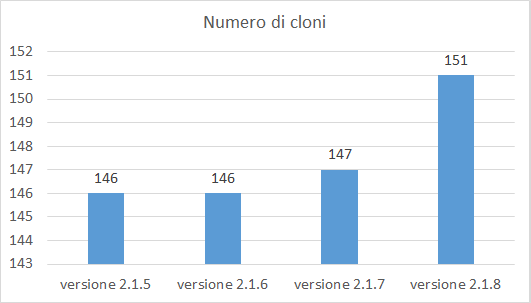
\includegraphics[scale=0.75, trim = 0cm 0cm 0cm 0cm, clip=true]{Grafici_dnsJava/NumeroCloni.png}
	\caption{Analisi numero cloni DnsJava}
	\label{fig:nCloniDnsJava}
\end{figure}
\begin{figure}[h]
	\centering
	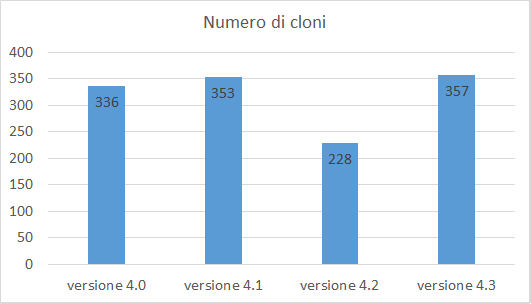
\includegraphics[scale=0.75, trim = 0cm 0cm 0cm 0cm, clip=true]{Grafici_jabRef/NumeroCloni.png}
	\caption{Analisi numero cloni JabRef}
	\label{fig:nCloniJabRef}
\end{figure}
\begin{figure}[h]
	\centering
	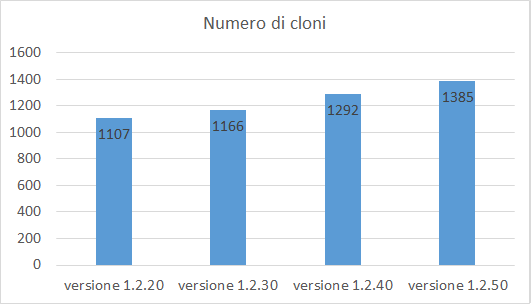
\includegraphics[scale=0.75, trim = 0cm 0cm 0cm 0cm, clip=true]{Grafici_fastJson/NumeroCloni.png}
	\caption{Analisi numero cloni FastJson}
	\label{fig:nCloniFastjson}
\end{figure}
Si nota dunque che l'unico dato anomalo si ha sulla versione $4.2$ di JabRef in cui il numero di cloni diminuisce rispetto alla versione precedente. Questo risultato non va però ad inficiare il trend verificato nelle analisi degli altri progetti in quanto si nota che nella versione $4.3$ vi è non solo un aumento rispetto alla versione $4.2$, ma addirittura un incremento rispetto a tutte le precedenti versioni. 

La seconda analisi ha riguardato il \textbf{numero di cloni di ogni tipo} per le $4$ versioni di ciascuno dei progetti presi in considerazione. In linea di massima, il numero di cloni di tipo $3$ è sempre maggiore rispetto a quello dei cloni di tipo $1$ e $2$. In particolare:
\begin{itemize}
	\item in \textbf{DnsJava}, come mostrato in \autoref{fig:tipiCloniDnsJava}, si hanno:
		\begin{itemize}
				\item versione $2.1.5$: 7 cloni di tipo 1, 27 cloni di tipo 2, 112 di tipo 3;
				\item versione $2.1.6$: 7 cloni di tipo 1, 27 cloni di tipo 2, 112 di tipo 3;
				\item versione $2.1.7$: 7 cloni di tipo 1, 27 cloni di tipo 2, 113 di tipo 3;
				\item versione $2.1.8$: 9 cloni di tipo 1, 27 cloni di tipo 2, 115 di tipo 3;		
		\end{itemize}
	\item in \textbf{JabRef}, come mostrato in \autoref{fig:tipiCloniJabRef}, si hanno:
				\begin{itemize}
			\item versione $4.0$: 8 cloni di tipo 1, 48 cloni di tipo 2,280 di tipo 3;
			\item versione $4.1$: 10 cloni di tipo 1, 49 cloni di tipo 2, 294 di tipo 3;
			\item versione $4.2$: 2 cloni di tipo 1, 20 cloni di tipo 2, 206 di tipo 3;
			\item versione $4.3$: 8 cloni di tipo 1, 49 cloni di tipo 2, 300 di tipo 3;		
		\end{itemize}
	\item in \textbf{FastJson}, come mostrato in \autoref{fig:tipiCloniFastjson}, si hanno:
	\begin{itemize}
		\item versione $1.2.20$: 270 cloni di tipo 1, 120 cloni di tipo 2,717 di tipo 3;
		\item versione $1.2.30$: 284 cloni di tipo 1, 140 cloni di tipo 2, 742 di tipo 3;
		\item versione $1.2.40$: 301 cloni di tipo 1, 150 cloni di tipo 2, 841 di tipo 3;
		\item versione $1.2.50$: 313 cloni di tipo 1,154 cloni di tipo 2, 918 di tipo 3;		
	\end{itemize}
\end{itemize}
Quello che si nota è quindi che in tutti i progetti analizzati il numero di cloni di tipo 3 è predominante. I cloni di tipo 2 sono maggiori rispetto a quelli di tipo 1 tranne che in \textbf{FastJson}, essendo quest'ultima una libreria.
\begin{figure}[h]
	\centering
	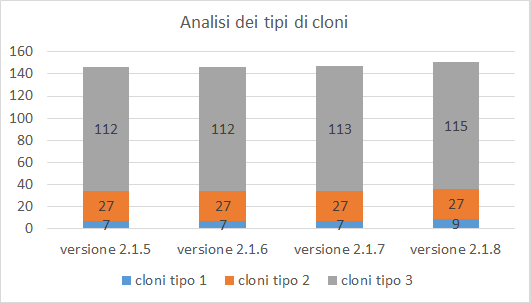
\includegraphics[scale=0.75, trim = 0cm 0cm 0cm 0cm, clip=true]{Grafici_dnsJava/TipiCloni.png}
	\caption{Analisi tipo cloni DnsJava}
	\label{fig:tipiCloniDnsJava}	
\end{figure}
\begin{figure}[h]
	\centering
	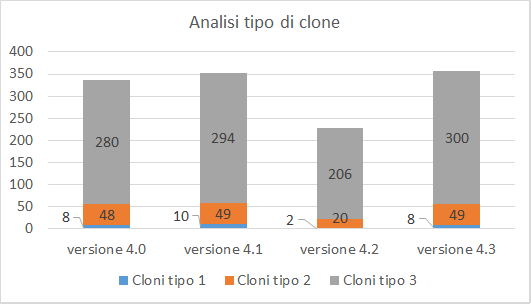
\includegraphics[scale=0.75, trim = 0cm 0cm 0cm 0cm, clip=true]{Grafici_jabRef/TipiCloni.png}
	\caption{Analisi tipo cloni JabRef}
	\label{fig:tipiCloniJabRef}
\end{figure}
\begin{figure}[h]
	\centering
	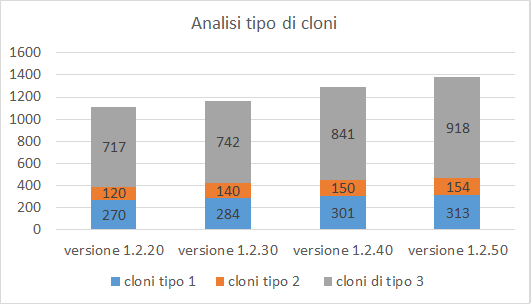
\includegraphics[scale=0.75, trim = 0cm 0cm 0cm 0cm, clip=true]{Grafici_fastJson/TipiCloni.png}
	\caption{Analisi tipo cloni FastJson}
	\label{fig:tipiCloniFastjson}
\end{figure}

Procedendo nell'analisi è stato individuato il numero di file in cui sono presenti cloni differenziandoli quindi da quelli in cui i cloni non compaiono:
\begin{itemize}
	\item in \textbf{DnsJava}, come mostrato in \autoref{fig:percentualeDnsJava} si hanno:
	\begin{itemize}
		\item versione 2.1.5: 60 file con cloni e 129 senza cloni;
		\item versione 2.1.6: 60 file con cloni e 130 senza cloni;
		\item versione 2.1.7: 61 file con cloni e 134 senza cloni;
		\item versione 2.1.8: 65 file con cloni e 131 senza cloni;
	\end{itemize}
	\item in \textbf{JabRef}, come mostrato in \autoref{fig:percentualeJabRef}, si hanno:
	\begin{itemize}
		\item versione 4.0: 156 file con cloni e 1373 senza cloni;
		\item versione 4.1: 158 file con cloni e 1409 senza cloni;
		\item versione 4.2: 76 file con cloni e 1618 senza cloni;
		\item versione 4.3: 160 file con cloni e 1542 senza cloni;
	\end{itemize}
		\item in \textbf{FastJson}, come mostrato in \autoref{fig:percentualeFastjson}, si hanno:
	\begin{itemize}
		\item versione 1.2.20: 480 file con cloni e 1473 senza cloni;
		\item versione 1.2.30: 510 file con cloni e 1639 senza cloni;
		\item versione 1.2.40: 576 file con cloni e 1908 senza cloni;
		\item versione 1.2.50: 598 file con cloni e 2047 senza cloni;
	\end{itemize}
\end{itemize}
A partire dai dati raccolti sono state considerate le percentuali di file con cloni e senza cloni, notando che si ha una maggiore percentuale di file senza cloni. La minore percentuale di file con cloni sul totale si ha in jabRef.
\begin{figure}[h]
	\centering
	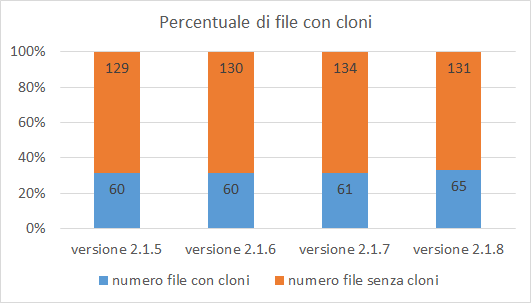
\includegraphics[scale=0.75, trim = 0cm 0cm 0cm 0cm, clip=true]{Grafici_dnsJava/PercentualeFileCloni.png}
	\caption{Analisi percentuale file con e senza cloni DnsJava}
	\label{fig:percentualeDnsJava}	
\end{figure}
\begin{figure}[h]
	\centering
	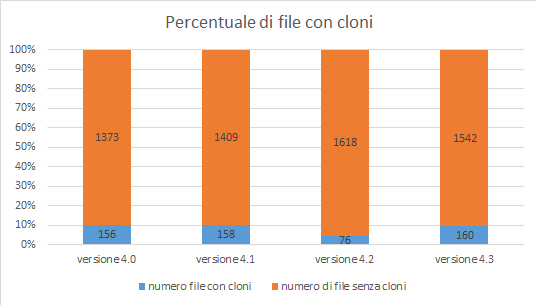
\includegraphics[scale=0.75, trim = 0cm 0cm 0cm 0cm, clip=true]{Grafici_jabRef/PercentualeFileCloni.png}
	\caption{Analisi percentuale file con e senza cloni JabRef}
	\label{fig:percentualeJabRef}
\end{figure}
\begin{figure}[h]
	\centering
	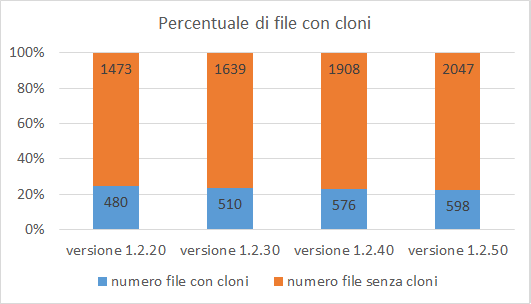
\includegraphics[scale=0.75, trim = 0cm 0cm 0cm 0cm, clip=true]{Grafici_fastJson/PercentualeFileCloni.png}
	\caption{Analisi percentuale file con e senza cloni FastJson}
	\label{fig:percentualeFastjson}
\end{figure}
Si è proceduto all'analisi della presenza di code smell nei file con e senza cloni considerando i valori medi. In particolare:
\begin{itemize}
	\item in DnsJava, come mostrato in \autoref{fig:codeSmellDnsJava}:
	\begin{itemize}
		\item versione 2.1.5: in media, il numero di code smell è 63 nei file senza cloni e 209 in quelli con i cloni;
		\item versione 2.1.6: in media, il numero di code smell è 63 nei file senza cloni e 213 in quelli con i cloni;
		\item versione 2.1.7: in media, il numero di code smell è 61 nei file senza cloni e 220 in quelli con i cloni;
		\item versione 2.1.8: in media, il numero di code smell è 61 nei file senza cloni e 219 in quelli con i cloni;
	\end{itemize}
	\item in JabRef, come mostrato in \autoref{fig:codeSmellJabRef}:
	\begin{itemize}
		\item versione 4.0: in media, il numero di code smell è 36 nei file senza cloni e 156 in quelli con i cloni;
		\item versione 4.1: in media, il numero di code smell è 41 nei file senza cloni e 148 in quelli con i cloni;
		\item versione 4.2: in media, il numero di code smell è 38 nei file senza cloni e 155 in quelli con i cloni;
		\item versione 4.3: in media, il numero di code smell è 38 nei file senza cloni e 88 in quelli con i cloni;
	\end{itemize}
	\item in FastJson, come mostrato in \autoref{fig:codeSmellFastjson}:
	\begin{itemize}
		\item versione 1.2.20: in media, il numero di code smell è 30 nei file senza cloni e 125 in quelli con i cloni;
		\item versione 1.2.30: in media, il numero di code smell è 28 nei file senza cloni e 138 in quelli con i cloni;
		\item versione 1.2.40: in media, il numero di code smell è 28 nei file senza cloni e 177 in quelli con i cloni;
		\item versione 1.2.50: in media, il numero di code smell è 30 nei file senza cloni e 184 in quelli con i cloni;
	\end{itemize}
\end{itemize}
Si è visto che nei file contenenti cloni, il numero medio di code smell è in generale maggiore rispetto al caso in cui il file non contiene i cloni stessi. La differenza risulta maggiormente evidente in \textbf{FastJson}.
\begin{figure}[h]
	\centering
	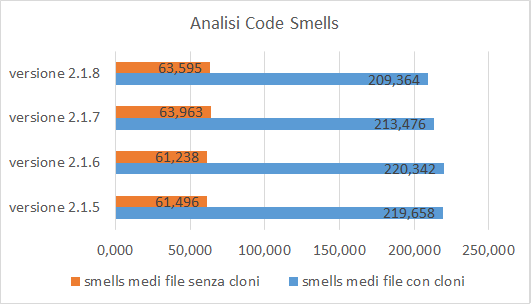
\includegraphics[scale=0.75, trim = 0cm 0cm 0cm 0cm, clip=true]{Grafici_dnsJava/CodeSmells.png}
	\caption{Numero medio code smell file con e senza cloni DnsJava}
	\label{fig:codeSmellDnsJava}	
\end{figure}
\begin{figure}[h]
	\centering
	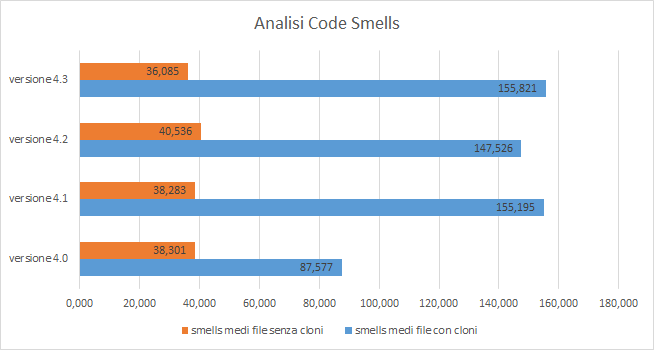
\includegraphics[scale=0.75, trim = 0cm 0cm 0cm 0cm, clip=true]{Grafici_jabRef/CodeSmells.png}
	\caption{Numero medio code smell file con e senza cloni JabRef}
	\label{fig:codeSmellJabRef}
\end{figure}
\begin{figure}[h]
	\centering
	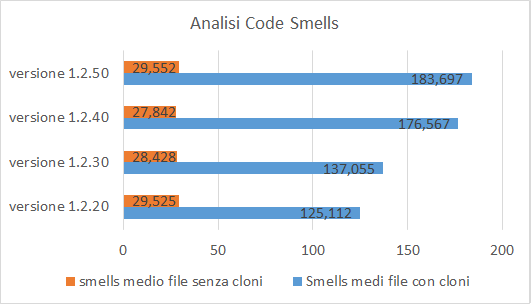
\includegraphics[scale=0.75, trim = 0cm 0cm 0cm 0cm, clip=true]{Grafici_fastJson/CodeSmell.png}
	\caption{Numero medio code smell file con e senza cloni FastJson}
	\label{fig:codeSmellFastjson}
\end{figure}
La stessa analisi è stata effettuata prendendo in considerazione il technical debt. In particolare sono stati ottenuti i seguenti risultati:
\begin{itemize}
		\item in DnsJava, come mostrato in \autoref{fig:tdDnsJava}:
	\begin{itemize}
		\item versione 2.1.5: in media, il techical debt è di 319 minuti nei file senza cloni e 1240 minuti in quelli con i cloni;
		\item versione 2.1.6: in media, il techical debt è di è 321 minuti nei file senza cloni e 1267 in quelli con i cloni;
		\item versione 2.1.7: in media, il techical debt è di 291 minuti nei file senza cloni e 1330 minuti in quelli con i cloni;
		\item versione 2.1.8: in media, il techical debt è di 292 nei file senza cloni e 1327 in quelli con i cloni;
	\end{itemize}
	\item in JabRef, come mostrato in \autoref{fig:tdJabRef}:
	\begin{itemize}
		\item versione 4.0: in media, il techical debt è di 177 minuti nei file senza cloni e 1104 minuti in quelli con i cloni;
		\item versione 4.1: in media, il techical debt è di 177 minuti nei file senza cloni e 1109 minuti in quelli con i cloni;
		\item versione 4.2: in media, il techical debt è di 185 minuti nei file senza cloni e 1232 in quelli con i cloni;
		\item versione 4.3: in media, il techical debt è di 163 nei file senza cloni e 1090 in quelli con i cloni;
	\end{itemize} 
		\item in FastJson, come mostrato in \autoref{fig:tdFastjson}:
	\begin{itemize}
		\item versione 1.2.20: in media, il techical debt è di 130 minuti nei file senza cloni e 655 in quelli con i cloni;
		\item versione 1.2.30: in media, il techical debt è di 124 minuti nei file senza cloni e 727 minuti in quelli con i cloni;
		\item versione 1.2.40: in media, il techical debt è di 122 minuti nei file senza cloni e 1047 in quelli con i cloni;
		\item versione 1.2.50: in media, il techical debt è di 125 minuti nei file senza cloni e 1143 in quelli con i cloni;
	\end{itemize}
\end{itemize}
Si nota quindi che il tempo necessario per gestire e quindi manutenere una classe in cui sono presenti dei cloni, è più alto rispetto al caso in cui nella classe non risultano presenti i cloni stessi. Al fine di validare tale risultato, è stata effettuata un'analisi ulteriore. In particolare, per ogni versione di ogni progetto, è stato considerato il rapporto tra code smell e techical debt. I risultati ottenuti sono i seguenti:
%%%ANALISI RAPPORTO%%%%
\begin{itemize}
	\item in DnsJava, come mostrato in \autoref{fig:rapDnsJava}, il rapporto tra technical debt e code smell è pari a circa 4 minuti nel caso di file senza cloni e a 5 nel caso di file con cloni in tutte e tre le versioni;
	\item in JabRef, come mostrato in \autoref{fig:rapJabRef}, il rapporto risulta circa pari a 4 nel caso di file senza cloni in tutte e tre le versioni. Nel caso di file con cloni il rapporto risulta circa pari a 7 nelle versioni 4.0 , 4.1 e 4.3 mentre risulta pari a 8 nel caso della versione 4.2;
	\item in FastJson, come mostrato in \autoref{fig:rapFastjson} il rapporto risulta essere pari a circa 4 minuti nel caso di file senza cloni e a 5 minuti nel caso di file con cloni in tutte e 4 le versioni.
\end{itemize}
I risultati evidenziano quindi che la presenza di cloni influisce sia sulla quantità di code smell che sul technical debt mostrando quindi che i cloni stessi impattano sulla presenza di altri code smell.
\begin{figure}[h]
	\centering
	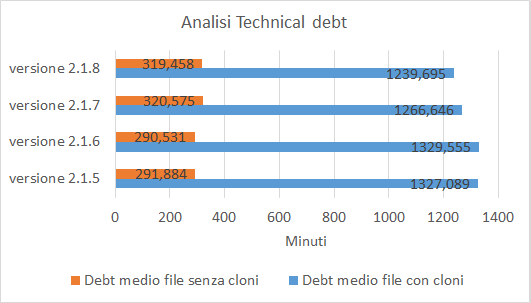
\includegraphics[scale=0.75, trim = 0cm 0cm 0cm 0cm, clip=true]{Grafici_dnsJava/TechnicalDebt.png}
	\caption{Techical Debt medio file con e senza cloni DnsJava}
	\label{fig:tdDnsJava}	
\end{figure}
\begin{figure}[h]
	\centering
	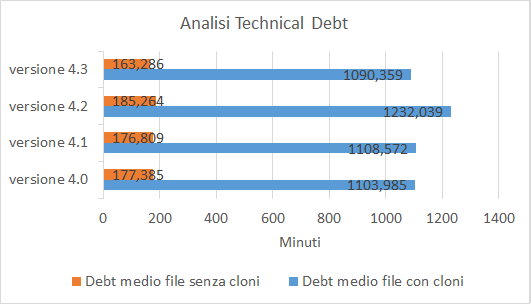
\includegraphics[scale=0.75, trim = 0cm 0cm 0cm 0cm, clip=true]{Grafici_jabRef/TechnicalDebt.png}
	\caption{Techical Debt medio file con e senza cloni JabRef}
	\label{fig:tdJabRef}
\end{figure}
\begin{figure}[h]
	\centering
	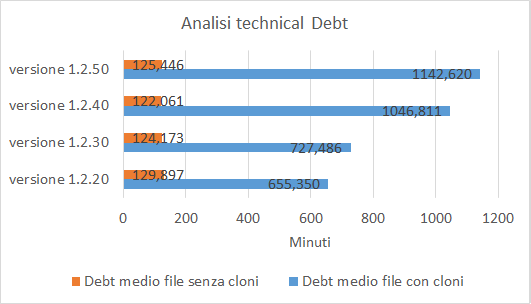
\includegraphics[scale=0.75, trim = 0cm 0cm 0cm 0cm, clip=true]{Grafici_fastJson/TechnicalDebt.png}
	\caption{Techical Debt medio file con e senza cloni FastJson}
	\label{fig:tdFastjson}
\end{figure}

%%%%%%%%%%%%%%%%%%%%%%%%%%%%%%%%%%%
\begin{figure}[htbp]
	\centering
	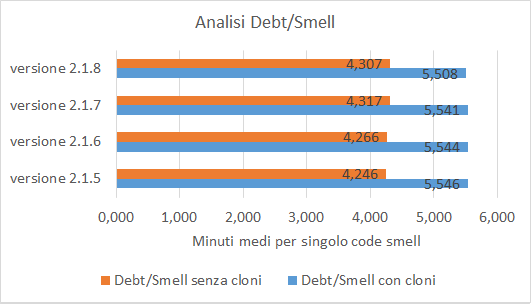
\includegraphics[scale=0.75, trim = 0cm 0cm 0cm 0cm, clip=true]{Grafici_dnsJava/Debt-Smell.png}
	\caption{Rapporto $\frac{code smell}{technical debt}$ file con e senza cloni DnsJava}
	\label{fig:rapDnsJava}	
\end{figure}
\begin{figure}[htbp]
	\centering
	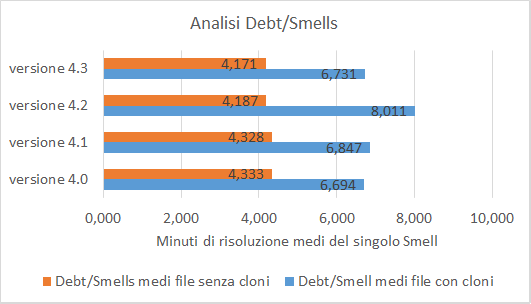
\includegraphics[scale=0.75, trim = 0cm 0cm 0cm 0cm, clip=true]{Grafici_jabRef/Debt-Smells.png}
	\caption{Rapporto $\frac{code smell}{technical debt}$ file con e senza cloni JabRef}
	\label{fig:rapJabRef}
\end{figure}
\begin{figure}[htbp]
	\centering
	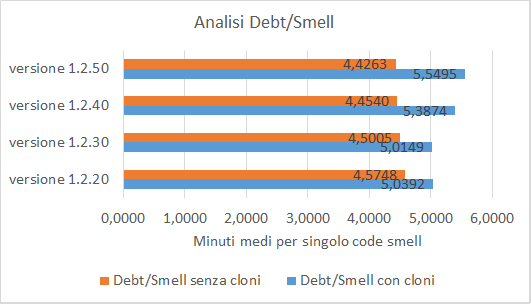
\includegraphics[scale=0.75, trim = 0cm 0cm 0cm 0cm, clip=true]{Grafici_fastJson/Debt-Smell.png}
	\caption{Rapporto $\frac{code smell}{technical debt}$ file con e senza cloni FastJson}
	\label{fig:rapFastjson}
\end{figure}

\chapter{Conclusioni}\label{cap5}



\end{document}